\documentclass[a0paper,landscape,fontscale=0.285]{baposter}

\usepackage{setspace}
\usepackage{graphicx}

\usepackage{tikz}
\usepackage{pgfbaselayers}
\pgfdeclarelayer{background}
\pgfdeclarelayer{foreground}
\pgfsetlayers{background,main,foreground}

%%% Color Definitions %%%%%%%%%%%%%%%%%%%%%%%%%%%%%%%%%%%%%%%%%%%%%%%%%%%%%%%%%

\definecolor{bordercol}{RGB}{40,40,40}
\definecolor{headercol1}{RGB}{186,215,230}
\definecolor{headercol2}{RGB}{80,80,80}
\definecolor{headerfontcol}{RGB}{0,0,0}
\definecolor{boxcolor}{RGB}{186,215,230}


%%% Utility functions %%%%%%%%%%%%%%%%%%%%%%%%%%%%%%%%%%%%%%%%%%%%%%%%%%%%%%%%%%

%%% Save space in lists. Use this after the opening of the list %%%%%%%%%%%%%%%%
\newcommand{\compresslist}{
        \setlength{\itemsep}{1pt}
        \setlength{\parskip}{0pt}
        \setlength{\parsep}{0pt}
}

\usepackage{polyglossia}
\setdefaultlanguage[variant=australian]{english}

\usepackage{fontspec}
\defaultfontfeatures{PunctuationSpace=3,Scale=MatchLowercase,Mapping=tex-text}
\newfontfeature{IPA}{+mgrk}
%\setromanfont[IPA]{FreeSerif}
%\setromanfont[IPA,Scale=0.8]{CMU Serif}
\setromanfont[IPA]{Liberation Serif}
%\setromanfont[IPA]{Times New Roman}
%\setromanfont[IPA]{NimbusRomNo9L-Regu}
%\setromanfont{Times New Roman}
\setmonofont[IPA]{Liberation Mono}
%\renewcommand{\sfdefault}{phv}
%\renewcommand{\rmdefault}{ptm}
%\renewcommand{\ttdefault}{pcr}
\usepackage[small,bf]{caption}
%\newfontfamily\qipa[IPA]{NimbusRomNo9L-Regu}
\newfontfamily\qipa[IPA,Scale=MatchLowercase]{FreeSerif}
%\newfontfamily\htwo[IPA,Scale=1.2]{FreeSans}
\newfontfamily\htwo[IPA,Scale=1.2]{CMU Sans Serif}
\newfontfamily\titlefont[IPA]{CMU Serif}

% FIXME: Breaks baposter
%\usepackage[novoc,fdf2alif]{arabxetex}
%\newfontfamily\uighurfont[Script=Arabic,Scale=1.5]{Lateef}
%\newfontfamily\arabicfont[Script=Arabic,Scale=1.5]{Lateef}

\usepackage{natbib}

%\usepackage[in]{fullpage}
\usepackage[colorlinks=true,citecolor=black,linkcolor=black,urlcolor=blue]{hyperref}

\usepackage{subfigure}
\usepackage{booktabs}

%%\bibpunct{(}{)}{;}{A}{,}{,}
%\bibdata{paper}

\newcommand{\citemultileft}[1]{(\citeauthor{#1}, \citeyear{#1}}
\newcommand{\citemultimid}[1]{\citeauthor{#1}, \citeyear{#1}}
\newcommand{\citemultiright}[1]{\citeauthor{#1}, \citeyear{#1})}
\newcommand{\citetwoyears}[2]{\citeauthor{#1} (\citeyear{#1} and \citeyear{#2})}

% for glosses
\newcommand{\eng}[1]{`{\em #1}'}
%dammit, sc doesn't seem to be working
\newcommand{\gmk}[1]{\textsc{#1}}

\newenvironment{itemise}[1]{
        \begin{itemize}\setlength{\itemsep}{-0.2em}
        \vspace{-0.5em}
        #1
}{
        \end{itemize}
        \vspace{-2pt}
}

%\newcommand{\h2}[1]{{\big



\begin{document}
	% To get it to be A0 consistently on all machines..
	\special{papersize=1189mm,841mm}
	\setlength{\pdfpageheight}{\paperheight}
	\setlength{\pdfpagewidth}{\paperwidth}

%%% Setting Background Image %%%%%%%%%%%%%%%%%%%%%%%%%%%%%%%%%%%%%%%%%%%%%%%%%%
%\background{
%	
\includegraphics[width=0.99\textwidth]{flagkg2}
%}
	\background{{
		\begin{tikzpicture}[remember picture,overlay]%
			\draw (current page.north west)+(-4em,2em) node[anchor=north west] {
\includegraphics[width=1.1\textwidth,height=1.1\textheight]{flagkg2}};
		\end{tikzpicture}%
%		
\includegraphics[width=0.99\textwidth]{flagkg2}
%			\draw (current page.north west)+(-2em,2em) node[anchor=north west] {
\includegraphics[width=0.9\textwidth]{flagkg2}};
	}}



	\begin{poster}{
			grid=false,
			eyecatcher=false,
			borderColor=bordercol,
			headerColorOne=headercol1,
			headerColorTwo=headercol2,
			headerFontColor=headerfontcol,
			% Only simple background color used, no shading, so boxColorTwo isn't necessary
			boxColorOne=boxcolor,
			headershape=roundedright,
  headerborder=open,
  headerheight=0.08\textheight,
  %headershape=roundedright,
  %headershade=plain,
  %headerfont=\Large\textsf, %Sans Serif
			%headerfont=\Large\sf\bf,
			textborder=rectangle,
			%background=plain,
			background=user,
			headerborder=open,
			boxshade=plain,
			textborder=roundedleft,
		}{
			Eye Catcher, empty if option eyecatcher=false - unused
		}{
			{\vspace{0.5ex}
			{\titlefont \textsc{A finite-state morphological transducer for Kyrgyz}}}
		}{
			%Jonathan North Washington {\small (Indiana University, \texttt{jonwashi@indiana.edu})}, Mirlan Ipasov {\small (International Ataturk Alatoo University, \texttt{mipasov@gmail.com})}, Francis M.\ Tyers {\small (Universitat d'Alacant, \texttt{ftyers@dlsi.ua.es})}

			\vspace{-1.2em}
			{\begin{minipage}[t]{13em}
				\begin{spacing}{0.4}
					Jonathan North Washington\\
					{\small Indiana University, \texttt{jonwashi@indiana.edu}}
				\end{spacing}
			\end{minipage}
			\begin{minipage}[t]{17em}
				\begin{spacing}{0.4}
					Mirlan Ipasov\\
					{\small International Ataturk Alatoo University, \texttt{mipasov@gmail.com}}
				\end{spacing}
			\end{minipage}
			\begin{minipage}[t]{13em}
				\begin{spacing}{0.4}
					Francis M.\ Tyers\\
					{\small Universitat d'Alacant, \texttt{ftyers@dlsi.ua.es}}
				\end{spacing}
			\end{minipage}}

			%\begin{minipage}[c]{12em}
			%	\centering
			%	\begin{spacing}{0.4}
			%		Jonathan Washington\\
			%		Indiana University\\
			%		\texttt{jonwashi@indiana.edu}
			%	\end{spacing}
			%\end{minipage}
			%\begin{minipage}[c]{18em}
			%	\centering
			%	\begin{spacing}{0.4}
			%		Mirlan Ipasov\\
			%		International Ataturk Alatoo University\\
			%		\texttt{mipasov@gmail.com}
			%	\end{spacing}
			%\end{minipage}
			%\begin{minipage}[c]{10em}
			%	\centering
			%	\begin{spacing}{0.4}
			%		Francis M.\ Tyers\\
			%		Universitat d'Alacant\\
			%		\texttt{ftyers@dlsi.ua.es}
			%	\end{spacing}
			%\end{minipage}

			%Jonathan Washington, Mirlan Ipasov, Francis M.\ Tyers\\
			%Indiana University, Universitat d'Alacant, International Ataturk Alatoo University\\
			%\texttt{jonwashi@indiana.edu}, \texttt{mipasov@gmail.com}, \texttt{ftyers@dlsi.ua.es}
		}{
			%University Logo(s)
			{\begin{minipage}{19em}
				\hfill
				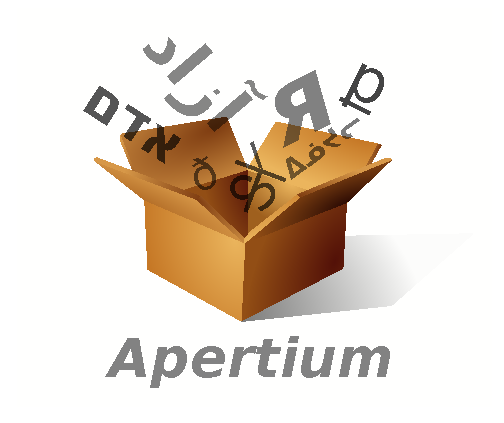
\includegraphics[height=6.5em]{apertium}
				
\includegraphics[height=6.5em]{flagkg1}
			\end{minipage}}
		}

		\headerbox{Overview}{name=overview,column=0,row=0}{
			\begin{spacing}{0.8}
This paper describes the development of a free/open-source finite-state morphological transducer for Kyrgyz. The transducer 
has been developed for morphological generation for use within a prototype Turkish$\rightarrow$Kyrgyz machine translation system, but has also been extensively tested for analysis. The finite-state toolkit used for the work was the Helsinki Finite-State 
Toolkit (HFST). The paper describes some issues in Kyrgyz morphology, the development of the tool, some linguistic issues encountered and how they were dealt with, and 
which issues are left to resolve. An evaluation is presented which shows that the transducer has medium-level coverage, between 82\% and 87\% on two freely available corpora of Kyrgyz, and high precision and recall over a manually verified test set.
			\end{spacing}\vspace{-0.25ex}
		}
		\headerbox{Kyrgyz}{name=kyrgyz,below=overview}{
* Kyrgyz\\
		}
		\headerbox{Morphological Transducers}{name=morphtrans,below=kyrgyz}{
* Morphological transducers\\
		}
		\headerbox{Available Turkic Transducers}{name=turkictrans,below=morphtrans}{
* Other Turkic morphological transducers\\
		}
		\headerbox{Framework: HFST / Apertium}{name=framework,below=turkictrans}{
* HFST/Apertium
		}

		\headerbox{The Transducer}{name=transducer,column=1,span=2,row=0}{
Tagset\\
* something witty\\

Things we do well\\
* Morphophonology\\
** vowel harmony\\
** voicing assimilation\\
** desonorisation\\
* N-N compounds (чакыруу кагазы) ?
		}

		\headerbox{Evaluation}{name=coverage,span=2,column=1,below=transducer}{
			{\htwo Test corpora}
			\begin{itemise}
				\item \textbf{Kyrgyz Wikipedia} dump dated 2011-09-23 (\texttt{kywiki-20110923-pages-articles.xml})
				\item All 2010 articles from \textbf{Radio Free Europe / Radio Liberty} (RFE/RL)'s Kyrgyz service (\texttt{azattyk.org})
				\item both split into 10 equal parts; coverage calculated over each separately; standard deviation of the mean was calculated
			\end{itemise}
			%both split into 10 equal parts; coverage calculated over each separately; standard deviation of the mean was calculated\\
			{\htwo Two measures}
			\begin{itemise}
				\item \textbf{Naïve coverage} - the percentage of surface forms in a given corpus that receive at least one analysis\\(forms counted by this measure may have other analyses which are not delivered by the transducer)
				\item \textbf{Mean ambiguity} - the average number of analyses for each surface form encountered when analysing this corpus
			\end{itemise}
			{\htwo Evaluation Results (as of revision \texttt{r36739})}\\
\centering
\vspace{1pt}\hspace{2em}
			%\begin{centering}
			{\large
				\begin{tabular}{lrrrr}
					\toprule
					Corpus           & Tokens    & Known       & Naïve coverage (\%) & Mean ambiguity\\
					\midrule 
					Kyrgyz Wikipedia & 329,524   & 270,668     & 82.1 $\pm$ 3.2      & 2.35\\
					RFE/RL Kyrgyzstan & 4,112,558 & 3,614,193   & 87.9 $\pm$ 1.2      & 2.43\\
					\bottomrule
				\end{tabular}
			}
			%\end{centering}
		}

		\headerbox{Недостатки}{name=nedostatki,column=3,row=0}{
Things we don't do [well [yet]]\\
* case changes for words with one root (Финландия / финландиялык)\\
* abbreviations (АКШнын) and numbers ({\qipa 100дүн})\\
* compound verbs\\
* gerunds with mono-syllabic V-final verbs (*жөө / жеш < же-)
		}

		\headerbox{References}{name=references,column=3,below=nedostatki}{
%			\begin{thebibliography}{1}\itemsep=-0.01em
%			\setlength{\baselineskip}{0.4em}
%
		}


	\end{poster}
\end{document}
